\documentclass[sigconf,anonymous,review]{acmart}

\settopmatter{printacmref=true, printccs=true, printfolios=true}
\renewcommand\footnotetextcopyrightpermission[1]{}
\pagestyle{plain}
\acmConference[SCORED '26]{Workshop on Software Supply Chain Offensive Research and Ecosystem Defenses}{October 6, 2026}{Prague, Czech Republic}

\usepackage{amsmath}
\usepackage{booktabs}
\usepackage{enumitem}
\usepackage{mathtools}
\usepackage{microtype}
\usepackage{tikz}
\usepackage{xspace}
\usetikzlibrary{arrows.meta,positioning,fit}

\newcommand{\sys}{\textsc{GlueRift}\xspace}
\newcommand{\result}{\mathsf{Result}}
\newcommand{\ok}{\mathsf{Ok}}
\newcommand{\err}{\mathsf{Err}}
\newcommand{\safe}{\mathsf{Safe}}
\newcommand{\matchrel}{\mathsf{Match}}
\newcommand{\sound}{\mathsf{Sound}}
\newcommand{\adequate}{\mathsf{Adequate}}
\newcommand{\precise}{\mathsf{Precise}}
\newcommand{\faithful}{\mathsf{Faithful}}
\newcommand{\defined}{\mathsf{Defined}}
\newcommand{\lawful}{\mathsf{Lawful}}
\newcommand{\all}{\mathsf{All}}
\newcommand{\yes}{\textsf{P}}
\newcommand{\no}{\textsf{D}}
\newcommand{\na}{\textsf{--}}

\title{Round Trips Can Lie: Policy-Laundering Attacks on Cross-Language Validation Adapters}

\begin{document}

\begin{abstract}
A recent Go-to-Rust validation architecture first checks adapter
round trips and then reuses the adapters to compare program outputs.
Even exhaustive round-trip checks do not establish semantic alignment.
Over a shared total bijective carrier domain, conjugating one endpoint's
adapter by a carrier permutation preserves native, carrier-domain, and full
cross-language round trips, yet can make a
source \texttt{DENY} transport to the same target-native value as a
target \texttt{ALLOW}.  We call this a policy-laundering attack.

We present \sys, a finite checker that treats the workflow's
target-native comparator as a first-class input.  It separates policy soundness,
which forbids unsafe induced equalities, from comparison adequacy,
which requires declared matches to compare equal.  Precision and
faithfulness expose extra equality and exact realization.  This
two-sided criterion rejects both false agreement and vacuous
always-different adapters.  The checker uses closed adapter and
observer languages, exhaustively decides supported finite scopes,
classifies generated transformations, and returns concrete paths and
witnesses; unsupported semantics are reported as unknown.

We mechanize the total finite core in Lean and evaluate four distinct
law-preserving attacks, benign and vacuity regressions, and total
composition.  Two separate-process Go/Rust replays through a shared
Protobuf carrier reproduce target-native false agreement: an enum
decision reversal and a nested repeated-type field-role swap.  All six
round trips pass in both.  A direct-relation baseline, given the same
semantics, reaches exactly the same top-level verdicts and first
witnesses.  Thus our contribution is not a new lens law or a logically
stronger relation checker; it is an operational attack on a concrete
validation seam and a reproducible diagnostic realization.
\end{abstract}

\begin{CCSXML}
<ccs2012>
 <concept>
  <concept_id>10002978.10003029.10003032</concept_id>
  <concept_desc>Security and privacy~Formal security models</concept_desc>
  <concept_significance>500</concept_significance>
 </concept>
 <concept>
  <concept_id>10011007.10011006.10011041</concept_id>
  <concept_desc>Software and its engineering~Software verification and validation</concept_desc>
  <concept_significance>500</concept_significance>
 </concept>
</ccs2012>
\end{CCSXML}
\ccsdesc[500]{Security and privacy~Formal security models}
\ccsdesc[500]{Software and its engineering~Software verification and validation}
\keywords{translation validation, interoperability, round trips, policy laundering, bidirectional transformations}

\maketitle

\section{Introduction}

Cross-language validation needs a way to compare values that do not
share a native representation.  This is especially difficult for
opaque, library-defined values.  A recent Go-to-Rust translation
pipeline synthesizes Go and Rust adapters around a shared Protobuf
carrier, checks source-side and full cross-language round trips, and
then reuses those adapters for differential I/O comparison
\cite{zhang2026validated}.  For a source function $f$, target function
$g$, and input/output adapters $A_I,A_O$, the final test is
$A_O(f(v))=g(A_I(v))$ on observed test inputs.  Round-trip success is
therefore admission evidence for glue that later participates in the
equivalence verdict.

The motivating workflow checks a Go-side round trip and a full
Go-to-Rust-to-Go round trip on representative values.  Our counterexample
strengthens, rather than weakens, this admission criterion: the reference
artifact checks both native laws, both carrier-domain laws, and both full
transports exhaustively over declared finite domains.  The attack therefore
does not depend on asymmetric or sampled round-trip testing.

This evidence leaves an ambiguity.  For a permutation $\sigma:C\to C$,
the conjugated target maps $\sigma\circ e_T$ and $d_T\circ\sigma^{-1}$
insert a change and its inverse into every cycle.  In this shared bijective
core they cancel, so every round trip still passes.
They need not cancel at the downstream comparison boundary.  The
twisted decoder may transport a source denial to the target's allowed
constructor; if the target program also returns that allowed value,
the validator reports equality between policy-opposite executions.

This is not a claim that round-trip ambiguity or automorphism
invariance is new.  Lens research supplies round-trip laws,
consistency relations, quotients, contracts, and composition
\cite{foster2007lenses,hofmann2011symmetric,foster2008quotient,zhang2023contract,xia2019monadic}.
Cycle-consistency theory gives a closely related automorphism
ambiguity \cite{moriakov2020cyclegan}, and language-interoperability
research verifies glue conversion relative to an independently stated
semantic relation \cite{patterson2022semantic}.  Our question is more
operational and narrower:

\begin{quote}
Can glue admitted by all ordinary adapter round trips cause the
\emph{workflow's target-native comparison cut} in a cross-language validation
workflow to report unsafe program agreement?
\end{quote}

We answer yes with a theorem, finite generated attacks, and native
replays.  We then ask what additional evidence excludes the attack
without accepting the opposite vacuity---an adapter that never equates
anything.  \sys uses endpoint-owned relations: $\safe$ describes pairs
that may safely compare equal, while $\matchrel$ describes pairs that
must compare equal.  Their two inclusions define soundness and
adequacy.  The validator comparator is explicit: carrier equality,
source-native equality, and target-native equality are different
relations and no bridge is assumed between them.

This paper makes six contributions:

\begin{enumerate}[leftmargin=*,nosep]
  \item We exhibit a target-native policy-laundering attack in which
  six exhaustive round trips pass but the validator reports unsafe
  equality.
  \item We give a comparator-indexed formalization that separates
  soundness, adequacy, precision, and faithfulness over a declared
  validation scope.
  \item We characterize lawful twists and distinguish policy harm from
  transformations that merely break a requested law.
  \item We implement a closed finite checker that generates structural
  attacks, reports concrete witnesses and adapter paths, and returns
  unknown rather than approximating unsupported semantics.
  \item We mechanize nine theorem and counterexample groups in Lean and
  provide two separate-process Go/Rust/Protobuf replays.
  \item We compare against an equally expressive direct-relation
  baseline and require verdict and first-witness parity.
\end{enumerate}

We do not claim a vulnerability in the motivating authors' public
implementation, which we did not execute.  Our native experiments are
an architecture-path-faithful reconstruction of the adapter and comparator
topology.  Nor do we claim arbitrary
native-code verification, whole-program equivalence, attack
prevalence, or completeness beyond the declared finite language.

\section{The Validation Seam}
\label{sec:seam}

\subsection{Architecture and threat model}

Let $S$, $T$, and $C$ be finite source-native, target-native, and
carrier domains.  An adapter context contains four partial maps:
\begin{align*}
e_S &: S\to\result(C), & d_S &: C\to\result(S),\\
e_T &: T\to\result(C), & d_T &: C\to\result(T).
\end{align*}
The motivating output comparison transports a source output through
$e_S$ and $d_T$, then compares the resulting target-native value with
the target program's output.  Figure~\ref{fig:seam} shows the seam.

\begin{figure}[t]
\centering
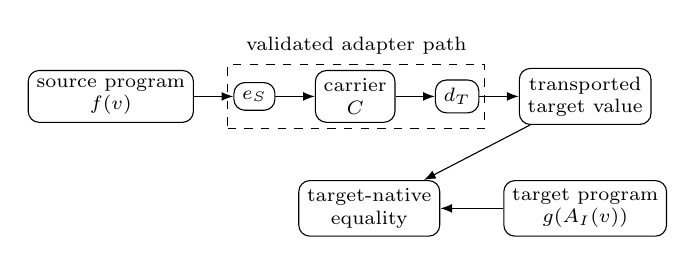
\begin{tikzpicture}[
  node distance=5mm and 5mm,
  box/.style={draw,rounded corners,align=center,inner sep=3pt,font=\scriptsize},
  arr/.style={-{Latex[length=1.5mm]},thin},
  every node/.style={font=\scriptsize}]
  \node[box] (sprog) {source program\\$f(v)$};
  \node[box,right=of sprog] (es) {$e_S$};
  \node[box,right=of es] (carrier) {carrier\\$C$};
  \node[box,right=of carrier] (dt) {$d_T$};
  \node[box,right=of dt] (transport) {transported\\target value};
  \node[box,below=7mm of transport] (tprog) {target program\\$g(A_I(v))$};
  \node[box,left=8mm of tprog] (cmp) {target-native\\equality};
  \draw[arr] (sprog)--(es);
  \draw[arr] (es)--(carrier);
  \draw[arr] (carrier)--(dt);
  \draw[arr] (dt)--(transport);
  \draw[arr] (transport)--(cmp);
  \draw[arr] (tprog)--(cmp);
  \node[draw,dashed,fit=(es)(carrier)(dt),inner sep=2pt,label={[font=\scriptsize]above:validated adapter path}] {};
\end{tikzpicture}
\caption{The target-native comparison seam.  Round trips validate the
adapter path; the final equality is between native target values.}
\Description{A source program output passes through a source encoder, a
shared carrier, and a target decoder. The transported target value is
compared for equality with the target program output.}
\label{fig:seam}
\end{figure}

The untrusted component is the adapter context: the four maps and any
carrier transformation.  The policy owner supplies finite comparison
domains, a pair universe $U\subseteq S\times T$, the comparator, and
endpoint semantics.  The adversary may choose a well-typed adapter
that passes all requested round trips, but cannot alter the comparator
or the endpoint policy.  This models an erroneous or adversarially
misaligned generated adapter, not a compromised compiler or program.

In the output-laundering fixtures, the source and target program bodies
and the input adapter are fixed; the input adapter is honest.  The target
program's permissive output is a pre-existing program disagreement.  The
adversarial output adapter does not create that disagreement: it causes the
validator to misclassify it as equality.

The Core is deliberately total on every admitted comparison and
round-trip input.  Object-language \texttt{Result} is an ordinary sum
whose branches may be permuted; meta-level conversion failure is not
silently ignored.  Effectful partial composition is outside our claims.

\subsection{The six round trips}

The request explicitly names six laws.  Native round trips require
\begin{align*}
d_S(e_S(s))&=\ok(s), & d_T(e_T(t))&=\ok(t).
\end{align*}
Carrier-domain round trips, on policy-owned $K_S,K_T\subseteq C$,
require
\begin{align*}
e_S(d_S(c))&=\ok(c) &&(c\in K_S),&
e_T(d_T(c))&=\ok(c) &&(c\in K_T).
\end{align*}
Full transports require the source-to-target-to-source and reverse
cycles to be defined and return their starting values:
\begin{align*}
d_S(e_T(d_T(e_S(s))))&=\ok(s),\\
d_T(e_S(d_S(e_T(t))))&=\ok(t).
\end{align*}
Composition above uses result binding; an intermediate error fails the
law.  A profile does not add laws implicitly.

These six laws are stronger than the sampled, Go-origin cycles in the
motivating workflow.  They are the reference artifact's admission request,
not a claim about which laws that workflow implements.

\subsection{A minimal laundering execution}

Take two source decisions, \texttt{DENY} and \texttt{ALLOW}, two target
decisions, \texttt{Blocked} and \texttt{Permitted}, and a two-value
carrier.  The aligned context maps denials to carrier 0 and allowances
to carrier 1.  Let $\sigma$ swap 0 and 1, and twist only the target
context:
\[
e_T^\sigma=\sigma\circ e_T,\qquad
d_T^\sigma=d_T\circ\sigma^{-1}.
\]
Then $d_T^\sigma(e_S(\texttt{DENY}))=\texttt{Permitted}$.  If the
source program denies and the target program permits, the transported
source output and target output are both \texttt{Permitted}.  The
ordinary comparator says equal even though the endpoint-owned policy
says the pair is unsafe.  Section~\ref{sec:evaluation} reproduces this
execution in separate Go and Rust processes through Protobuf.

The finite A01 instance makes every set explicit.  Its comparison universe
is the four-pair product
\[
U=\{\texttt{DENY},\texttt{ALLOW}\}\times
  \{\texttt{Blocked},\texttt{Permitted}\},
\]
and endpoint roles define
\[
\safe=\matchrel=
\{(\texttt{DENY},\texttt{Blocked}),
  (\texttt{ALLOW},\texttt{Permitted})\}.
\]
The aligned context induces exactly this relation.  The carrier swap instead
induces
\[
I_{A^\sigma}^T=
\{(\texttt{DENY},\texttt{Permitted}),
  (\texttt{ALLOW},\texttt{Blocked})\},
\]
so both induced pairs are unsafe while both required matches disappear.

\section{Comparator-Indexed Security}
\label{sec:model}

\subsection{Induced relations}

Carrier equality is not the comparison in Figure~\ref{fig:seam}.
Accordingly, the comparator specification chooses one of three induced
relations:
\begin{align}
E_A^C(s,t) &\iff \exists c.\ e_S(s)=\ok(c)=e_T(t),\label{eq:carrier}\\
E_A^T(s,t) &\iff e_S(s)\mathbin{\gg=}d_T=\ok(t),\label{eq:target}\\
E_A^S(s,t) &\iff e_T(t)\mathbin{\gg=}d_S=\ok(s).\label{eq:source}
\end{align}
The selected relation is $I_A^\chi=E_A^\chi\cap U$.  Comparator
definedness is a positive obligation over all of $U$; partial results
do not make implications vacuously true.

The three relations can differ despite all six round trips.  In our
V01 model, source and target encoders use disjoint carrier images, so
$E_A^C=\varnothing$, while both cross-decoders collapse the images to
the corresponding native values.  All six laws hold, yet
$E_A^T=E_A^S=\{(s_0,t_0),(s_1,t_1)\}$.  Thus carrier-based checking
would miss a native false agreement.  \sys checks the selected native
relation directly.  It produces a separate exhaustive bridge result
only when carrier summaries are reused for native claims.

\subsection{Safety, required matches, and two vacuities}

The policy owner declares
\[
\matchrel\subseteq\safe\subseteq U.
\]
$\safe(s,t)$ means that equating the pair is permitted by the security
policy.  $\matchrel(s,t)$ means that the validator is required to
equate it.  They induce four distinct checks:
\begin{align*}
\sound_\chi(A) &\iff I_A^\chi\subseteq\safe,\\
\adequate_\chi(A) &\iff \matchrel\subseteq I_A^\chi,\\
\precise_\chi(A) &\iff I_A^\chi\subseteq\matchrel,\\
\faithful_\chi(A) &\iff I_A^\chi=\matchrel.
\end{align*}
Soundness prevents unsafe false agreement.  Adequacy prevents an
always-different adapter from appearing safe.  Precision reports safe
but undeclared extra equality.  Faithfulness is exact comparison.

Coverage is not inferred from an adapter's successful image.  For
example, source-total coverage is
\[
\forall s\in D_S^{cmp}.\ \exists t\in D_T^{cmp}.\ (s,t)\in\matchrel,
\]
and target-total is symmetric; bidirectional-total requires both.
An empty $\matchrel$ under nonempty coverage makes the request invalid
before adapter properties are evaluated.  If the safety policy is
unconstrained (no safety dimensions, hence $\safe=U$), the checker
reports the vacuity and withholds a security certificate even though
the set inclusion for soundness is mathematically true.

Target non-amplification is one useful asymmetric safety instance.  If
policy levels form a checked finite preorder, it permits equality only
when the target is no more permissive than the source.  Its safe
transformations need not form a subgroup; Section~\ref{sec:twists}
keeps exact stabilizers separate from asymmetric safe sets.

\subsection{Shape checks, bridges, and certification}

The comparator choice also constrains the shape of a realizable
$\matchrel$.  Because encoders and decoders are deterministic,
$E_A^T$ is functional from source values to target values.  If the
source full-transport law holds over the comparison source domain, its
covered graph is also inverse-functional: two covered sources cannot
transport to the same target and then both return through the full
cycle.  The source-native case is symmetric.  Carrier equality becomes
a partial bijection when the corresponding native and carrier laws
hold on the admitted images.  \sys checks these comparator-specific
shape obligations before evaluating adequacy, so an impossible policy
request is invalid rather than an adapter failure.

Carrier evidence moves to a native claim only through an explicit
bridge.  For example, the carrier-to-target bridge over $U$ is
\[
\forall(s,t)\in U.\quad E_A^C(s,t)\Longleftrightarrow E_A^T(s,t).
\]
It is checked exhaustively and reported as proved, disproved, or
unknown.  The target-native property itself never depends on this
bridge: Equation~\eqref{eq:target} is evaluated directly.  Moreover,
bridge evidence belongs to one exact context.  A bridge for $A$ is not
reused after transforming the context to $A^\sigma$.

Certificates reflect the distinction among logical results.  A
diagnostic request cannot certify.  A policy-sound profile requires
soundness; a policy-sound-adequate profile requires both inclusions; a
faithful-exact profile additionally requires $\safe=\matchrel$ and the
declared coverage.  Any required law, definedness, coverage, anchor, or
property failure blocks certification.  An unconstrained safety policy
always blocks security certification.  These rules prevent a raw true
implication from being presented as stronger evidence than the policy
actually supplied.

\section{Law-Preserving Twists}
\label{sec:twists}

\subsection{Preservation and laundering}

Assume total mutually inverse maps $e_S:S\cong C:d_S$ and
$e_T:T\cong C:d_T$ over one shared carrier domain $C$, and a carrier
automorphism $\sigma:C\cong C$.  Define
$e_T^\sigma=\sigma\circ e_T$ and
$d_T^\sigma=d_T\circ\sigma^{-1}$; the source maps are unchanged.

\textbf{Theorem 1 (round-trip preservation).}
Under these assumptions, replacing the target maps by
$(e_T^\sigma,d_T^\sigma)$ preserves the source and target native round
trips, the source and target carrier round trips, and both full
cross-language transport round trips over $S$, $T$, and $C$.

\emph{Proof sketch.}  Source laws are unchanged.  Target native and carrier
laws follow from
\begin{align*}
d_T^\sigma\circ e_T^\sigma
 &=d_T\circ\sigma^{-1}\circ\sigma\circ e_T=d_T\circ e_T,\\
e_T^\sigma\circ d_T^\sigma
 &=\sigma\circ e_T\circ d_T\circ\sigma^{-1}=\mathsf{id}_C.
\end{align*}
The full transports require the endpoint carrier inverse laws, not only an
adjacent syntactic cancellation:
\begin{align*}
RT_{STS}^\sigma
 &=d_S\circ\sigma\circ e_T\circ d_T\circ\sigma^{-1}\circ e_S\\
 &=d_S\circ\sigma\circ\mathsf{id}_C\circ\sigma^{-1}\circ e_S
  =\mathsf{id}_S,\\
RT_{TST}^\sigma
 &=d_T\circ\sigma^{-1}\circ e_S\circ d_S\circ\sigma\circ e_T\\
 &=d_T\circ\sigma^{-1}\circ\mathsf{id}_C\circ\sigma\circ e_T
  =\mathsf{id}_T.
\end{align*}
The Lean development proves these clean total-domain statements.
\hfill$\square$

The executable checker does not infer this theorem outside the clean core;
for partial carrier domains it rechecks every request-scoped law exhaustively.
Equation~\eqref{eq:target} nevertheless becomes
\[
E_{A^\sigma}^T(s,t)\iff
d_T(\sigma^{-1}(e_S(s)))=t,
\]
so the target-native graph may change.

\par\filbreak\noindent
\textbf{Corollary 2 (request-scoped policy laundering).}
Under Theorem~1, let $\mathcal R$ be a valid request whose required law
set is contained in the six laws above.  If the declared family admits the
normalized automorphism $\sigma\in\Sigma_{\mathcal F}(A)$ with its inverse
and action domain $C$, and there exists $(s,t)\in U$ such that
$E_{A^\sigma}^\chi(s,t)$ and $\neg\safe(s,t)$, then
\[
\sigma\in\mathsf{HarmfulTrans}_{\chi,\mathcal F}(A,\mathcal R).
\]

The algebra is familiar from automorphism ambiguity; the security
content is the independently owned unsafe witness at the comparator
specified for program agreement.

\subsection{Lawfulness is request-scoped}

Not every transformation candidate is an attack.  For the finite normalized
candidate set $\Sigma_{\mathcal F}(A)$ admitted by a declared family and a
request $\mathcal R$, \sys first defines
\begin{align*}
\sigma\in\lawful_{\chi,\mathcal F}(A,\mathcal R)\iff {}&
\mathsf{WT}(A^\sigma)\land\mathsf{Inverse}(\sigma)\\
&\land\mathsf{Conjugated}(A,A^\sigma)\\
&\land\defined_\chi(A^\sigma,U)\\
&\land\bigwedge_{\ell\in\mathsf{Laws}(\mathcal R)}
  \mathsf{Holds}_\ell(A^\sigma).
\end{align*}
It then partitions candidates into \emph{lawful-safe},
\emph{lawful-harmful}, and \emph{law-breaking-or-inapplicable}.
The last bucket prevents a sound transformation that breaks a carrier
round trip from being reported as safe, and prevents a law-breaking
candidate from being advertised as a laundering attack.

Formally, the two lawful buckets are
\begin{align*}
\mathsf{SafeTrans}_{\chi,\mathcal F}
 &=\{\sigma\in\lawful_{\chi,\mathcal F}(A,\mathcal R)
     \mid\sound_\chi(A^\sigma)\},\\
\mathsf{HarmfulTrans}_{\chi,\mathcal F}
 &=\{\sigma\in\lawful_{\chi,\mathcal F}(A,\mathcal R)
     \mid\neg\sound_\chi(A^\sigma)\},\\
\mathsf{InapplicableTrans}_{\chi,\mathcal F}
 &=\Sigma_{\mathcal F}(A)\setminus
   \lawful_{\chi,\mathcal F}(A,\mathcal R).
\end{align*}
Thus ``harmful''
means a concrete unsafe equality under a candidate that still meets the
validator's admission request, not merely a malformed conversion.

Only when a structural subfamily $G_{\mathcal F}(A)\subseteq
\Sigma_{\mathcal F}(A)$ has separately established group laws do exact
endpoint-label-preserving permutations form the ordinary stabilizer subgroup.
We make no subgroup
claim for asymmetric policy.  Our T01 counterexample uses three
positions with source levels $(deny,allow,allow)$ and target levels
$(deny,deny,allow)$.  Two carrier permutations are each lawful-safe,
while their composition remains lawful under all six laws and becomes
harmful only because it maps target $allow$ to source $deny$.

\section{GlueRift}
\label{sec:system}

\subsection{Closed finite semantics}

\sys is a reference checker, not a verifier for arbitrary Go or Rust.
The Core type language contains unit, Boolean, bounded integers,
bit-vectors, sums, products, and object-language \texttt{Result}.
Adapters include identity and composition; enum, field, and result
branch permutations; structural sum/product maps; bounded complement;
and modular affine maps.  Observers include constructor and field
roles, finite policy maps, tuples, and cases.  Relations are exact
equality, validated finite-preorder non-amplification, or an explicitly
enumerated finite table.

\begin{table}[t]
\caption{Minimal Core boundary.}
\label{tab:ir}
\centering
\scriptsize
\setlength{\tabcolsep}{3.5pt}
\begin{tabular}{p{.19\columnwidth}p{.72\columnwidth}}
\toprule
Layer & Supported Core forms\\
\midrule
Types & Unit, Bool, bounded integer, bit-vector, sum, product, object Result\\
Adapters & Identity, compose, enum/field/result permutations, structural maps, complement, modular affine\\
Observers & Constructor/field role, finite policy map, tuple, case\\
Relations & Exact, checked finite preorder, finite table\\
Decision & Exhaustive over declared finite scope; unsupported is unknown\\
Composition & Total-success exact and finite-preorder judgments\\
\bottomrule
\end{tabular}
\end{table}

All types are enumerated canonically.  One semantic kernel evaluates
the four maps, three comparators, six laws, policy relations, coverage,
four comparison properties, transformations, and witnesses.  Anchor
coverage conservatively includes every reachable constructor or field
path read by any adapter map or active observer; only policy-owned
explicit irrelevance can remove a path.  A request outside the closed
observer language returns \textsf{unknown}, as tested by V06.

The structural analyzer enumerates equal-signature enum variants,
same-typed fields, compatible result branches, and their nested
compositions.  Bounded complement and modular affine maps are admitted
declared scalar candidates, not claimed to be automatically or
completely discovered.  For every generated attack the evidence binds
the aligned base context, normalized transformation and inverse,
$\all(C)$, the four mechanically conjugated maps, transformed context,
requested laws, classification, and first harmful witness.

\subsection{Composition boundary}

The Core composes only total-success observer judgments.  Relative to
domains $D_X,D_Y$ and observers $o_X,o_Y$, write
\[
\Gamma\vdash f:X\xrightarrow{R}Y
\]
when, for every $x\in D_X$, evaluation returns some $y\in D_Y$ such
that $f(x)=\ok(y)$ and $R(o_X(x),o_Y(y))$.  Exact obligations compose
by transitivity.
Non-amplification obligations compose only after the finite relation is
exhaustively checked reflexive and transitive.  Global observers are
discharged directly unless their structure is syntactically derivable.
C01 checks both exact and preorder composition.  We do not claim
effectful or partial-error composition.

\subsection{Mechanization and baselines}

The Lean 4 development contains nine checked groups: encoder
injectivity from native round trips; twist preservation of native,
carrier, and full transport laws; direct target-native laundering;
soundness/adequacy vacuity and V01 divergence; comparator bridges;
native relation shape; exact stabilizers and asymmetric non-closure;
and total composition.  The release runs an axiom audit and rejects
\texttt{sorry} or \texttt{admit}.  This mechanizes the stated total
finite core; it does not formally verify the Rust checker or native
backends.

BL2 exhaustively checks the same six round trips but receives no
endpoint $\safe$ or $\matchrel$.  BL4 receives the same normalized
$(A,\chi,U,\safe,\matchrel)$, evaluator, totality, validity, coverage,
and witness order as \sys.  Therefore BL4 must produce the same common
verdicts and first policy/property witness.  This is intentional: a
complete direct relation checker is logically sufficient, so BL4 is a
semantic control realization rather than a performance baseline.  The
current release shares A02's semantic witness path and parity-checks C01's
derivation with BL4.  Its observed exclusive evidence is generated-twist
provenance, context-bound carrier diagnostics, and native binding---not
greater logical expressiveness.

\section{Evaluation}
\label{sec:evaluation}

We evaluate six questions: whether all-six-round-trip attacks exist at
the workflow's target-native comparison cut; whether two-sided checks expose
vacuity; whether
the closed checker gives actionable diagnostics; whether total
composition works; whether BL4 parity holds; and whether native
processes reproduce the reference relation.  All results below are
categorical exhaustive checks, not sampled measurements.  \textsf{P}
means proved exhaustive and \textsf{D} means disproved by a canonical
witness.

\subsection{Protocol and fixed oracles}

The evaluation registry and categorical expected matrix were fixed by
the artifact contract before implementation.  It contains four aligned
base/attack pairs, four benign modes, comparator and vacuity
regressions, three asymmetric-transformation runs plus one
law-breaking run, two composition modes, and two native bindings: 24
canonical checker runs in total.  A test failure cannot be repaired by
changing its expected category.  Each attack base and candidate use
identical types, comparator, $U$, policy, scope, requested laws, and
profile; the only semantic change is the evidence-bound conjugation.

The checker enumerates values, pairs, dimensions, and witnesses in a
canonical order.  The canonical result owner mechanically generates every
categorical result cell in Tables~\ref{tab:core}, \ref{tab:regressions},
\ref{tab:native}, and \ref{tab:bl4delta}; the manuscript inputs those generated
fragments directly.  BL4 invokes the same evaluator and witness order, rather
than an independent implementation that could diverge accidentally.  Native
replay reports bind the exact A01 or A02 candidate hash and are accepted only
after exhaustive backend truth-table conformance.  We ran the entire release
procedure from a clean external output root and regenerated it for byte
comparison against the checked release.

\subsection{Finite attacks and benign adapters}

Table~\ref{tab:core} covers four distinct IR-level attack families.  Each
aligned base context is defined, passes all six laws, and is faithful.
Each twisted candidate is mechanically bound to that base, remains
defined, passes all six laws, and is classified lawful-harmful.  BL2
accepts every attack because its entire criterion is round-trip
success.  Both \sys and BL4 disprove the four comparison properties
and return the same first witness.

\begin{table}[t]
\caption{Core attack and benign matrix.  RT summarizes all six laws;
S/A/P/F are soundness, adequacy, precision, and faithfulness.}
\label{tab:core}
\centering
\scriptsize
\setlength{\tabcolsep}{3.2pt}
\input{generated/core-results-table.tex}
\end{table}

The benign rows guard against an attack-only checker.  H01 accepts
different constructor names with aligned roles; H02 accepts a physical
field reorder with correct logical roles.  H04 is intentionally
asymmetric: a conservative target is faithful under non-amplification,
but under exact semantics it remains adequate while soundness,
precision, and faithfulness fail.  This confirms that the relations
measure different obligations rather than aliases for one verdict.

\subsection{Comparator and vacuity regressions}

Table~\ref{tab:regressions} isolates common specification and
classification errors.  V01 proves all six laws in both runs.  Carrier
equality finds no induced pairs and is sound; target-native equality
finds two pairs and exposes an unsafe one.  Its carrier-to-target bridge
is disproved, so carrier evidence is explanatory only.  V02 rejects an
empty required-match relation under nonempty coverage.  V10 is sound
and adequate but not precise or faithful, demonstrating extra safe
equality.  The policy-vacuity run satisfies the raw inclusion but is
marked policy-unconstrained and receives no certificate.

\begin{table}[t]
\caption{Regression outcomes.}
\label{tab:regressions}
\centering
\scriptsize
\setlength{\tabcolsep}{3.3pt}
\input{generated/regressions-table.tex}
\end{table}

T01 confirms that asymmetric safe transformations are not closed under
composition: both generators are lawful-safe, while their composition
still passes every requested law and becomes harmful only under the
policy.  T02 confirms the three-way partition: it is policy-sound but
fails a requested target-carrier law and is therefore never called
lawful-safe.  Structural enumeration automatically generates A01,
A02, and A05, including A02's nested path; A03 is explicitly recorded
as an admitted declared scalar candidate.

\subsection{Native target-native false agreement}

We implement architecture-path-faithful native fixtures using a shared
Protobuf schema, a Go source process, and a Rust target process.  The
processes execute with an empty-plus-whitelist environment, bound
inputs and executables, read-only source enforcement, and network
isolation.  The native harness reads a content-addressed bundle emitted by
the checker as its only semantic authority; the four map tables, complete
target-native relation, six staged law tables, and canonical witness have
zero mismatches.

Table~\ref{tab:native} shows the decisive executions.  E01's source
returns \texttt{DENY}; the target returns \texttt{Permitted}; and the
twisted output adapter transports the source result to
\texttt{Permitted}.  The target-native comparator therefore returns
\texttt{EQUAL}.  E02 is non-enum and nested: the source returns bounds
$\{minimum:0,maximum:2\}$, while target and transported source both
return $\{minimum:2,maximum:0\}$.  Its witness identifies
\texttt{output.policy.bounds.minimum}, expected role
\texttt{minimum}, and transported role \texttt{source.maximum}.  All
six declared round-trip laws pass in both fixtures, and policy soundness is
disproved.

\begin{table}[t]
\caption{Separate-process native replays.}
\label{tab:native}
\centering
\scriptsize
\setlength{\tabcolsep}{2.8pt}
\input{generated/native-table.tex}
\end{table}

Table~\ref{tab:fidelity} separates the topology we reproduce from features
we deliberately omit.  In particular, E02 uses finite integer fields rather
than opaque library wrappers, so these runs support an operational proof
witness for the comparison path, not broad practicality for library adapters.

\begin{table}[t]
\caption{Motivating workflow versus native reconstruction.}
\label{tab:fidelity}
\centering
\scriptsize
\setlength{\tabcolsep}{2.7pt}
\begin{tabular}{p{.42\columnwidth}p{.24\columnwidth}p{.25\columnwidth}}
\toprule
Property & Motivating workflow & Reconstruction\\
\midrule
Shared Protobuf carrier & yes & yes\\
Source output transported to target type & yes & yes\\
Final target-native equality & yes & yes\\
Separate Go/Rust execution & yes & yes\\
Adapter synthesis & LLM-generated & fixed finite IR\\
Opaque external-library values & central & not modeled\\
Round-trip coverage & sampled Go cycles & exhaustive six laws\\
\bottomrule
\end{tabular}
\end{table}

These executions establish the operational claim for our
reconstruction, not prevalence and not a vulnerability in a named
implementation.  They also show why the comparator index matters: the
observed equality is target-native, not an assumed carrier equality.

\subsection{Baseline and reproducibility results}

BL2 reports all six laws proved for every lawful attack and therefore
admits them at the round-trip layer.  BL4 is paired with every required
attack, benign, composition, and regression run.  Across all paired
runs, common validity, coverage, policy, TNA, and
four property verdicts match \sys, as does the first shared witness.
Table~\ref{tab:bl4delta} reports the concrete A02 evidence difference.  It
also records that the nested semantic witness path is shared, avoiding an
advantage claim from a deliberately degraded baseline.

\begin{table}[t]
\caption{Observed evidence on A02; BL4 is the Direct-Relation control.}
\label{tab:bl4delta}
\centering
\scriptsize
\setlength{\tabcolsep}{3pt}
\input{generated/bl4-delta-table.tex}
\end{table}

Starting from the source-only package, run these commands in order:
\begin{quote}
\small\texttt{./artifact/bootstrap-tools}\\[-2pt]
\texttt{./artifact/reproduce}
\end{quote}
The first provisions checksum/version-pinned tools and caches; the second
auto-selects source-only generation or checked-release verification, rebuilds
every proof, checker fixture, baseline, and native binary, validates the
acyclic evidence graph, and regenerates both the result owner and the TeX
fragments input above.  Verification mode additionally byte-compares the
complete regenerated graph.  The Lean audit covers L1--L9 without placeholders.
Table~\ref{tab:evidence-map} shows how the principal paper claims connect to
mechanization and executable evidence.

\begin{table}[t]
\caption{Claim-to-evidence map.}
\label{tab:evidence-map}
\centering
\scriptsize
\setlength{\tabcolsep}{2.7pt}
\begin{tabular}{p{.29\columnwidth}p{.13\columnwidth}p{.34\columnwidth}p{.15\columnwidth}}
\toprule
Paper claim & Lean & Checker evidence & Native\\
\midrule
RT preservation & L2/L3 & A01/02/03/05 six-law reports & E01/E02\\
Direct target equality & L4 & A01/02/03/05 target reports & E01/E02\\
Comparator divergence & L5/L6 & V01 & --\\
Vacuity and extra equality & L5 & V01.carrier, V02, policy-vacuity, V10 & --\\
Lawful classification & L8 & T01/T02 & --\\
Total composition & L9 & C01 & --\\
\bottomrule
\end{tabular}
\end{table}

\section{Discussion and Limitations}

\paragraph{What the result says.}
Round trips establish that conversions cancel along specified cycles.
They do not identify which endpoint meanings carrier positions should
represent, nor do they establish security of a different comparison
cut through the cycle.  Independently owned endpoint relations break
that ambiguity.  Soundness excludes unsafe equality; adequacy prevents
the defense from succeeding by making comparison useless.

\paragraph{Trusted base.}
The policy owner must correctly declare finite domains, $U$, $\safe$,
$\matchrel$, observers, comparator, and requested laws.  \sys checks
well-formedness, coverage, supported observer syntax, and finite
relation properties, but it does not infer endpoint meaning.  The Rust
evaluator, Lean compiler/kernel, native toolchains, Protobuf runtime,
and canonicalization/evidence scripts are also trusted according to
their roles.  The Lean theorems reduce confidence in the formal spine;
they do not verify the checker implementation.

\paragraph{Scope.}
Completeness is only for finite declared values, the closed adapter and
observer IR, and the registered transformation family.  Scalar
templates are admitted candidates, not exhaustively discovered.
Arbitrary callbacks, general list semantics, unbounded integers,
effectful composition, and arbitrary Go/Rust adapters are unsupported.
The checker reports unknown rather than approximating a missing
observer.  A passing result says only that the selected properties hold
for the selected comparator and declared scope; it is not whole-program
equivalence.

\paragraph{External validity.}
We study one recent architecture and two adapter-path-faithful native
reconstructions.  We neither measure prevalence nor search for natural
vulnerabilities.  The contribution survives that limitation because
the claim is an implication counterexample: ordinary round-trip
admission does not entail target-native policy soundness.  Broader
studies may establish how often this seam occurs, but are not evidence
needed for the theorem.

\paragraph{Disclosure and ethics.}
The experiments do not target a deployed service, use credentials, or
execute the motivating preprint's public implementation.  They expose
an architecture-level design weakness through a reconstruction.  Because no
public implementation was executed or named as affected, we classify the
result as a counterexample to an abstract validation architecture, not an
implementation vulnerability, and make no implementation-specific disclosure
claim.

\section{Related Work}

\paragraph{Translation validation and interoperability glue.}
The motivating 2026 preprint synthesizes Protobuf-backed adapters,
checks Go-side and full Go/Rust round trips, and reuses the adapters for
I/O comparison on observed tests \cite{zhang2026validated}.  We attack
that admission seam in a reconstruction; we do not dispute its broader
translation results.  Differential translation validators such as FLOURINE
and RustAssure compare source and translated behavior through concrete
fuzzing or symbolic execution \cite{eniser2024translating,bai2025rustassure}.
Our target is orthogonal: the adapter-mediated relation needed for such a
comparison can itself turn a program disagreement into equality while
satisfying its admission laws.  GlueTest uses language interoperability to run
source-language tests against translated code and explicitly notes
that the interoperability layer can introduce inconsistencies
\cite{abid2024gluetest}.  Patterson et al. instead start from declared
type convertibility and a semantic relation, then prove target-level
glue sound relative to it \cite{patterson2022semantic}.  That defense
principle subsumes our top-level direct relation check.  Our delta is
the round-trip-preserving target-native attack, two-sided vacuity
diagnostics, generated finite twists, and bound native replay.

\paragraph{Lenses and bidirectional programming.}
Classical lenses establish round-trip laws and compositional
bidirectional transformations \cite{foster2007lenses}.  Symmetric
lenses model consistency directly between two domains
\cite{hofmann2011symmetric}; quotient lenses state well-behavedness
modulo equivalence \cite{foster2008quotient}; contract lenses attach
predicates that support safe partial composition
\cite{zhang2023contract}.  Monadic formulations study effectful
composition \cite{xia2019monadic}, which our total Core intentionally
does not claim.  Optics and type equivalences connect reversible
programs and canonical equivalences \cite{carette2019optics}.  These
works make explicit that semantic consistency and composition are not
new contributions of \sys.  BL4 operationalizes this strongest prior
principle and is required to match our logical verdicts.

\paragraph{Cycle consistency and automorphisms.}
Moriakov et al. show that exact CycleGAN solutions are invariant under
automorphisms and characterize the solution space as a principal
homogeneous space \cite{moriakov2020cyclegan}.  Our conjugation theorem
has the same algebraic shape.  We do not claim the twist theorem as a
new abstract result.  We instantiate it at a cross-language program
comparison boundary, define harm relative to endpoint-owned security
semantics, and retain only transformations that remain applicable and
lawful for the validator's explicit request.

\section{Conclusion}

Adapter round trips can all be correct while the comparison they enable
is wrong.  A carrier twist and its inverse cancel inside native,
carrier, and full transport cycles, yet alter the target-native graph
used to declare program agreement.  \sys makes that graph explicit and
checks it against both a safety relation and a required-match relation,
thereby excluding unsafe false agreement without accepting vacuous
non-comparison.  Lean proofs, four finite attack families, a fair
direct-relation baseline, and two Go/Rust/Protobuf replays support this
bounded claim.  The practical lesson is simple: round-trip admission is
not semantic alignment evidence for a downstream comparator; that
alignment requires independently owned endpoint obligations.

\bibliographystyle{ACM-Reference-Format}
\bibliography{references}

\end{document}
